
\documentclass[a4paper, 12pt]{article}
\usepackage[portuguese]{babel}
\usepackage[utf8]{inputenc}
\usepackage[T1]{fontenc}
\usepackage{indentfirst}
\usepackage{graphicx}
\usepackage{fancyhdr}
\usepackage{float}
\usepackage{geometry}
\usepackage{caption}
\usepackage{blindtext}
\usepackage{fullpage,supertabular,alltt,latexsym,amsfonts,/Users/renatonobre/Documents/.pvs/pvs/pvs}
\geometry{left=25mm, top=25mm, right=25mm, bottom=25mm}
\DeclareGraphicsExtensions{.pdf,.png,.jpg,.jpeg}
\captionsetup{labelformat=empty}
\begin{document}
	\begin{titlepage}

		\newcommand{\HRule}{\rule{\linewidth}{0.5mm}}
		\centering
		\textsc{\LARGE Universidade de Brasília}\\[0.5cm]
		\includegraphics{logo.jpg}\\[0.5cm]
		\textsc{\Large Instituto de Ciências Exatas}\\[0.5cm]
		\textsc{\Large Departamento de Ciência da Computação}\\[0.5cm]
		\textsc{\Large Princípios de Visão Computacional - Turma ``A''}\\[0.5cm]
		\HRule \\[0.4cm]
		{ \huge \bfseries Projeto Demonstrativo 1}\\[0.2cm]
		\HRule \\[3.0cm]
		\begin{minipage}{0.4\textwidth}
			\begin{flushleft} \large
				\emph{Nome:}\\
				\emph{Khalil Carsten}\\
				\emph{Renato Nobre}\\
			\end{flushleft}
		\end{minipage}
		~
		\begin{minipage}{0.4\textwidth}
			\begin{flushright} \large
				\emph{Matrícula:}\\
				\textsc{15/0134495}\\
				\textsc{15/0146698}\\
			\end{flushright}
		\end{minipage}\\[6.0cm]
		\textsc{\large \centering 4 de Setembro de 2017}\\
	\end{titlepage}

	\section*{Introdução}

    Detecção de elementos em imagens é uma parte essencial de diversas aplicações de visão computacional. Imagens possuem diversos elementos de interesse que podem ser usados com o objetivo de detectar outros aspectos da imagem. Altura de objetos, altura, rotação e foco da câmera, e distancia entre objetos.

    O objetivo deste projeto foi achar a altura conhecida de um elemento na imagem para achar a altura de outros elementos. Para isso foi calculado pontos de fuga, retas de fuga, linha do horizonte, e matriz de rotações $R$ em cinco imagens diferentes. O processo detalhado será discutido abaixo.

    \section*{Desenvolvimento}

    \begin{figure}[H]
		\centering
		\includegraphics[width=0.68\linewidth]{nolines1.jpeg}
		\caption{Figura 1 - Rampa para o Departamento de Ciência da Computação}
	\end{figure}

    \begin{figure}[H]
		\centering
		\includegraphics[width=0.95\linewidth]{lines1.jpg}
		\caption{Linhas vermelhas representam as linhas de fuga; Linha azul clara a linha do horizonte; Linha azul escura a linha até a cabeça e pés das pessoas}
	\end{figure}

    \begin{figure}[H]
		\centering
		\includegraphics[width=0.68\linewidth]{nolines2.jpeg}
		\caption{Figura 2 - Departamento de Ciência da Computação}
	\end{figure}

    \begin{figure}[H]
		\centering
		\includegraphics[width=0.95\linewidth]{lines2.jpg}
		\caption{Linhas vermelhas representam as linhas de fuga; Linha azul clara a linha do horizonte; Linha azul escura a linha até a cabeça e pés das pessoas}
	\end{figure}

    \begin{figure}[H]
		\centering
		\includegraphics[width=0.68\linewidth]{nolines3.jpg}
		\caption{Figura 3 - Saída do Ceubinho}
	\end{figure}

    \begin{figure}[H]
		\centering
		\includegraphics[width=0.95\linewidth]{lines3.jpg}
		\caption{Linhas vermelhas representam as linhas de fuga; Linha azul clara a linha do horizonte; Linha azul escura a linha até a cabeça e pés das pessoas}
	\end{figure}

    \begin{figure}[H]
		\centering
		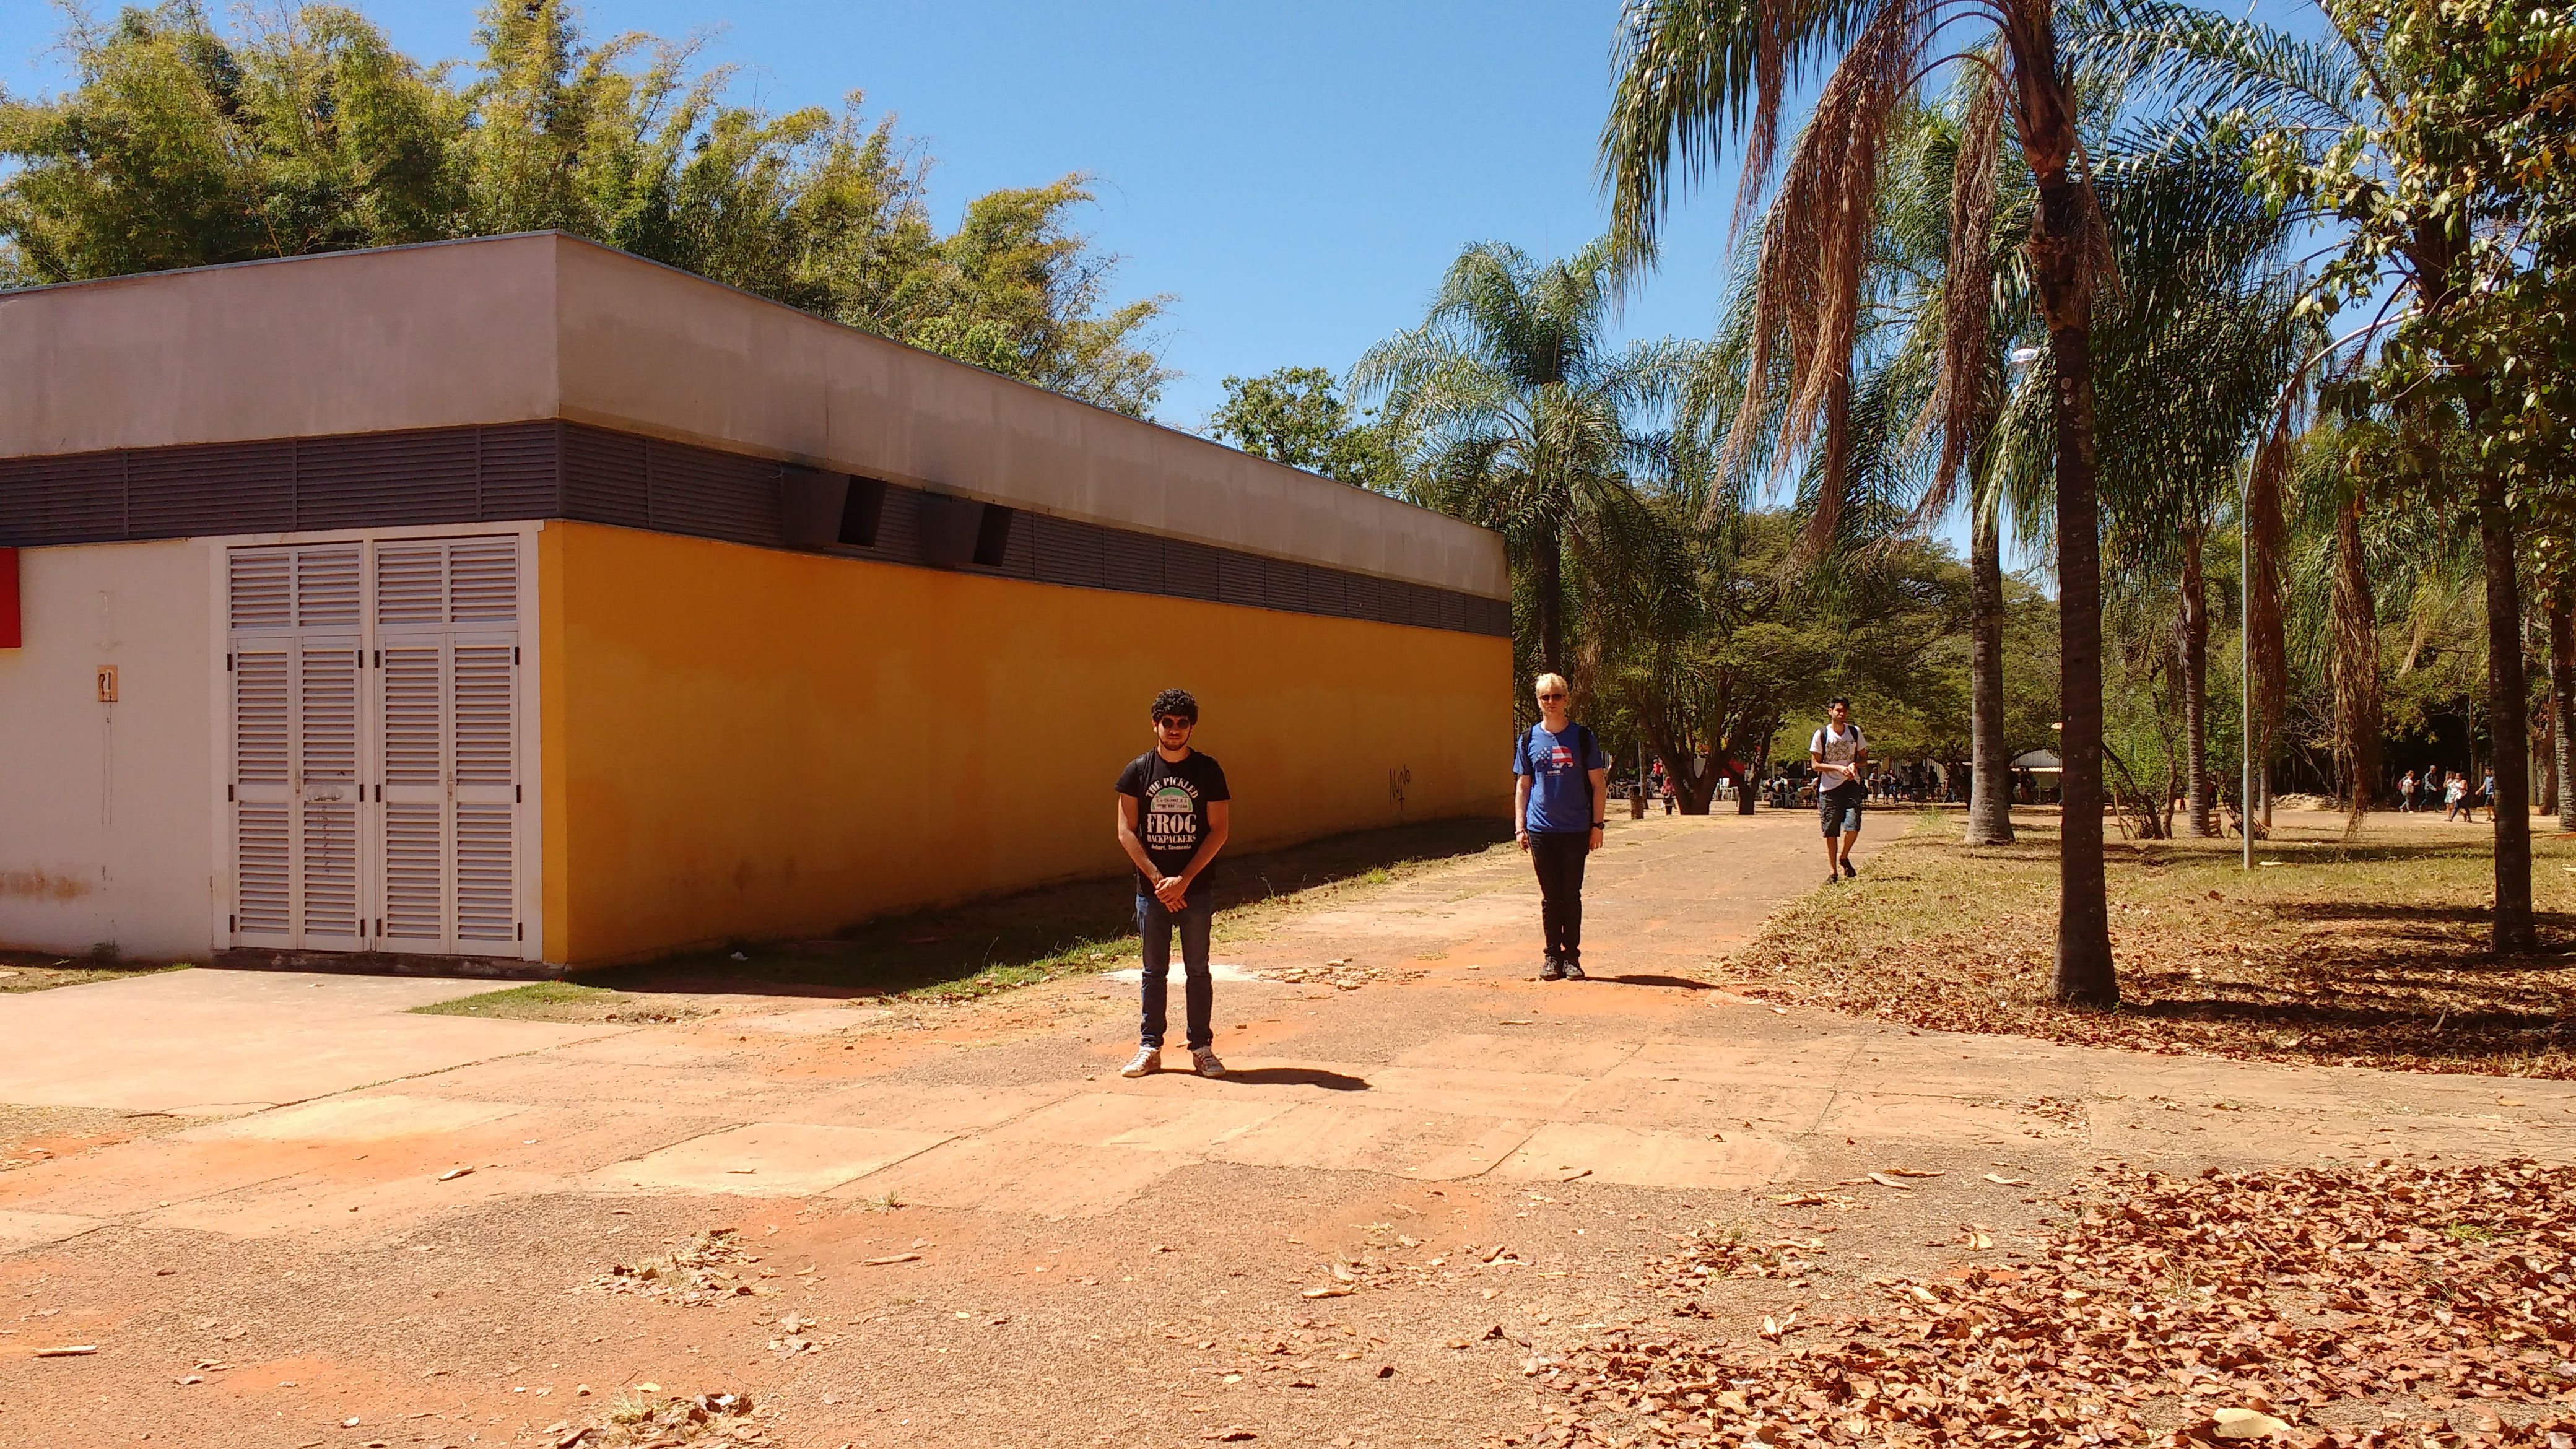
\includegraphics[width=0.68\linewidth]{nolines4.jpg}
		\caption{Figura 4 - Amarelinho do ICC Norte}
	\end{figure}

    \begin{figure}[H]
		\centering
		\includegraphics[width=0.95\linewidth]{lines4.jpg}
		\caption{Linhas vermelhas representam as linhas de fuga; Linha azul clara a linha do horizonte; Linha azul escura a linha até a cabeça e pés das pessoas}
	\end{figure}

    \begin{figure}[H]
        \centering
        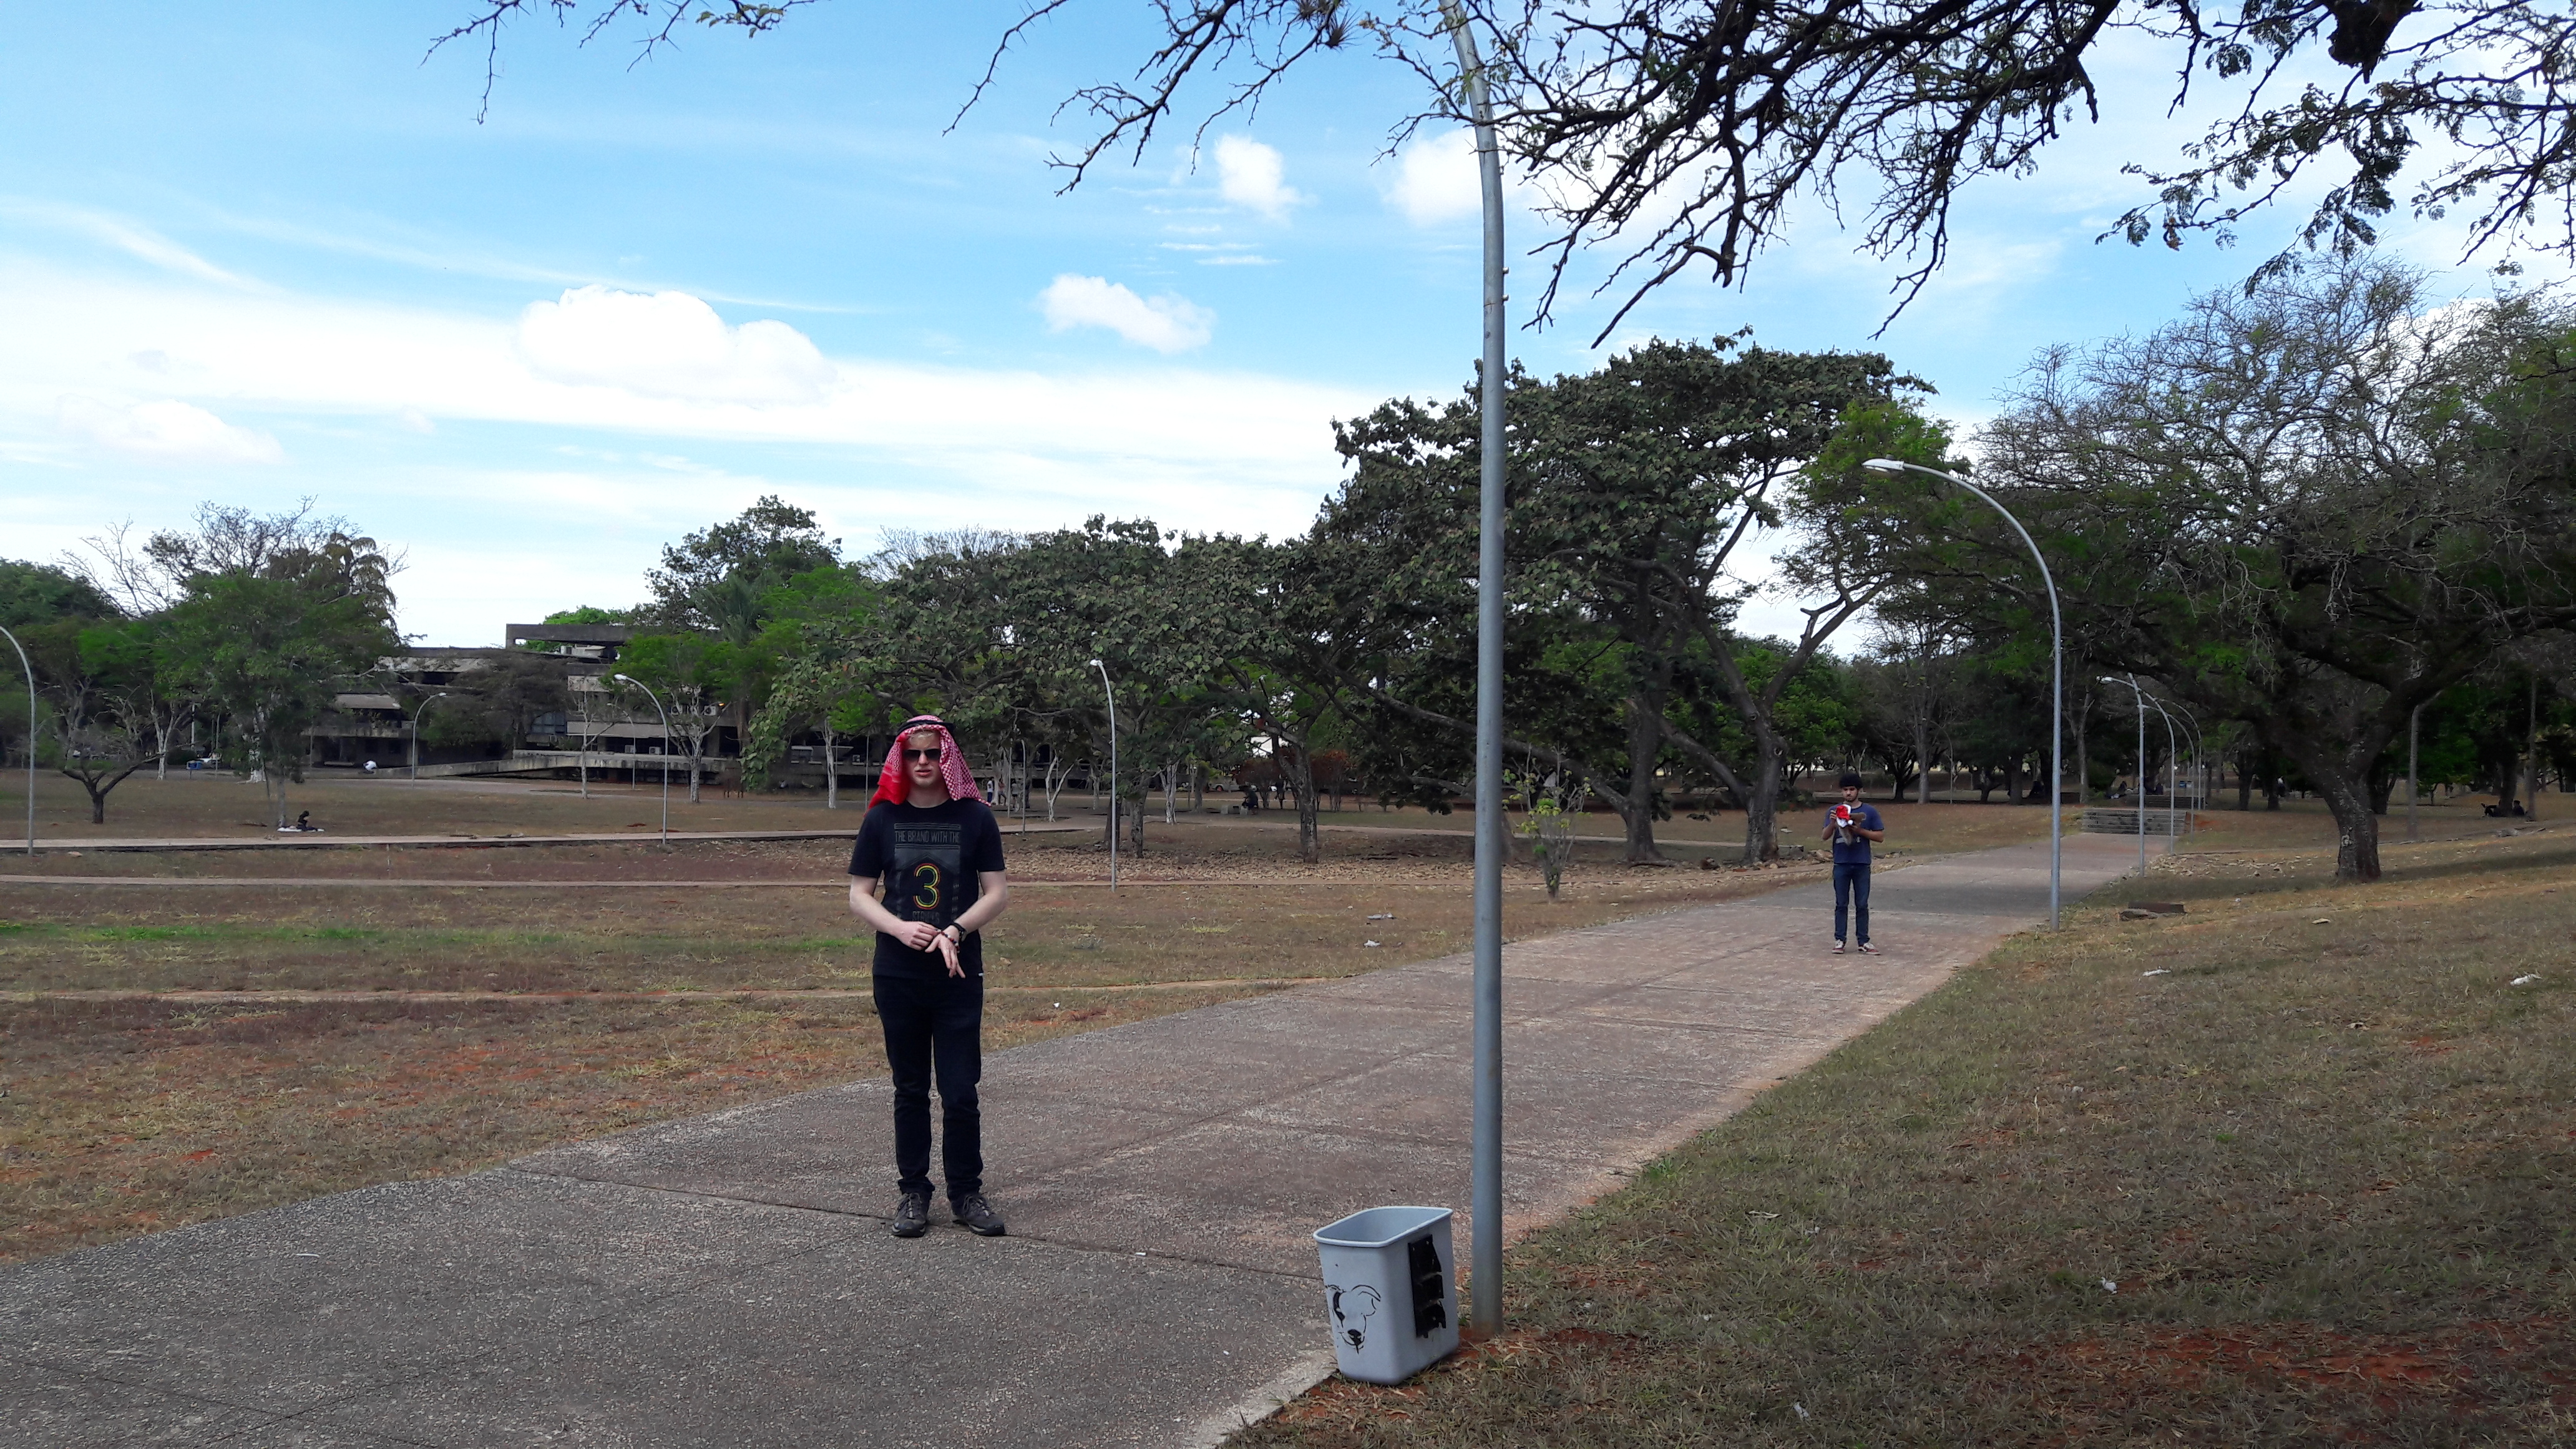
\includegraphics[width=0.68\linewidth]{nolines5.jpg}
        \caption{Figura 5 - Caminho Para a Reitoria}
    \end{figure}

    \begin{figure}[H]
        \centering
        \includegraphics[width=0.95\linewidth]{lines5.jpg}
        \caption{Linhas vermelhas representam as linhas de fuga; Linha azul clara a linha do horizonte; Linha azul escura a linha até a cabeça e pés das pessoas}
    \end{figure}


    \section*{Conclusão}
        O projeto realizado foi então validado comparando com a altura original das pessoas nas fotos a margem de erro é de aproximadamente 3 centímetros. A primeira pessoa que aparece nas duas primeiras imagens possui uma altura de $1.64$ metros, já a média da sua altura usando a altura encontrada nas as fotos foi de $1.61$ . Para a segunda pessoa, a média é de $1.72$, comparado com a altura real de $1.75$ metros.

        No entanto, o projeto apresenta certas dificuldades e limitações. Uma das principais dificuldades é em relação à disposição das fotos, que dependendo da maneira em que foi tirada pode se tornar impossível realizar os devidos cálculos. Outro ponto importante é que grande parte do projeto foi feito manualmente em vez de utilizar linhas de código para resolver o problema. Alguns passos podem ser automatizados, tais como, achar as linhas de fuga, o ponto de fuga, e detectar as pessoas nas imagens.

	\begin{thebibliography}{9}

        \bibitem{book1}
        Szeliski, Richard. ``Computer vision: algorithms and applications.'' Springer Science \& Business Media, 2010.

        \bibitem{slides}
        Slides de Aula


    \end{thebibliography}



\end{document}
